\documentclass[twocolumn, 9pt]{extarticle}
\usepackage{amsmath}
\usepackage{amssymb}
\usepackage{graphicx}
\usepackage{geometry}
\usepackage{hyperref}
\usepackage{bbm}
\geometry{a4paper, margin=0.7in}

\title{Multi-Agent Systems Exam\\
\small \href{https://github.com/ValentinisAlessio/MultiAgentSystems_Exam}{GitHub repository with the code}} %% Da capire dove mettere questo link
\author{Fantuzzi Giulio, Valentinis Alessio}
\date{June 18, 2025}

\begin{document}
\maketitle

\section{Parameter identification for DTMCs}

\subsection{Preliminaries}
We consider a DTMC with two states, $S = \{s_A, s_B\}$, and a parametric transition probability matrix $P = \begin{pmatrix} 1 - p & p \\ q & 1 - q \end{pmatrix}$, 
where $p$ and $q$ are the parameters to be identified.
The aim of the project is to estimate $p$ and $q$ based on a finite number of traces ($N$) of finite length ($n$), using different parameter inference techniques. In what
follows, we assume the initial distribution over the states to be known (\textit{e.g. uniformly distributed}), thus we focus on the estimation of the transition probabilities only.

\subsection{Methodology}
We explore two different approaches for parameter inference:
\begin{itemize}
    \item \textbf{Maximum Likelihood Estimation (MLE):} this method estimates the parameters by maximizing the likelihood of the observed data. 
    \item \textbf{Bayesian Inference:} this method estimates the posterior distribution of parameters, given a prior distribution and the observed data.
\end{itemize}
\subsubsection{Maximum Likelihood Estimation (MLE)}
In order to estimate the parameters $p$ and $q$ using MLE, we derive the likelihood function based on the observed traces.
Given a single trace $\sigma_i = s_1s_2\dots s_n$ of length $n$, its likelihood is given by the following expression:
\begin{align*}
L(\sigma_i \mid p, q) &= P(s_1) \prod_{j=1}^{n-1} P(s_{j+1} \mid s_j) \propto \prod_{j=1}^{n-1} P(s_{j+1} \mid s_j) \\
&= \prod_{j=1}^{n-1} [ \mathbbm{1}_{\{s_j = s_A,\, s_{j+1} = s_A\}} (1 - p) \cdot\\
&\quad  \mathbbm{1}_{\{s_j = s_A,\, s_{j+1} = s_B\}} p \cdot \\
&\quad  \mathbbm{1}_{\{s_j = s_B,\, s_{j+1} = s_A\}} q \cdot \\
&\quad  \mathbbm{1}_{\{s_j = s_B,\, s_{j+1} = s_B\}} (1 - q) ]
\end{align*}

Let $N_{ij}$ be the number of transitions from state $s_i$ to $s_j$ in the trace. An alternative formulation of the likelihood is:
\[
L(\sigma_i \mid p, q) = (1 - p)^{N_{AA}} p^{N_{AB}} q^{N_{BA}} (1 - q)^{N_{BB}}
\]

and the corresponding log-likelihood:
\begin{align*}
    l(\sigma_i \mid p, q) =& N_{AA} \log(1 - p) + N_{AB} \log(p) +\\
    &N_{BA} \log(q) + N_{BB} \log(1 - q)
\end{align*}

To obtain the Maximum Likelihood estimates, we need to maximize the log-likelihood function with respect to the parameters $p$ and $q$.
Since the two parameters are independent and depend only on the counts of transitions, we can maximize the log-likelihood function separately for each parameter.
\begin{align*}
    \begin{cases}
        \frac{\partial l}{\partial p} = \frac{N_{AB}}{p} - \frac{N_{AA}}{1 - p} = 0 &\Rightarrow \hat p = \frac{N_{AB}}{N_{AA} + N_{AB}} \\
        \frac{\partial l}{\partial q} = \frac{N_{BA}}{q} - \frac{N_{BB}}{1 - q} = 0 &\Rightarrow \hat q = \frac{N_{BA}}{N_{BA} + N_{BB}}
    \end{cases}
\end{align*}

We observe that these estimates are nothing but the relative frequencies of transitions from state $s_A$ to state $s_B$ and from state $s_B$ to state $s_A$, respectively.
\\

In terms of consistency, the ML estimates converge to the true parameters as the number of traces $N$ increases.
Let $p_{ij}^0$ be the true transition probabilities, and keep the same notation as above. Recall that
$\hat p_{ij} = \frac{N_{ij}}{\sum_j N_{ij}}$, with $N_{ij} = \sum_{i=1}^{n-1} \mathbbm{1}_{s=i}(s_t) \mathbbm{1}_{s=j}(s_{t+1})$.
It holds that:
\begin{align*}
    \frac{N_{ij}}{n-1} &= \frac{1}{n-1} \sum_{t=1}^{n-1} \mathbbm{1}_{s=i}(s_t) \mathbbm{1}_{s=j}(s_{t+1}) \\
    &\to_{n \to \infty} \mathbb{E} \left[ \mathbbm{1}_{s=i}(s_t) \mathbbm{1}_{s=j}(s_{t+1}) \right] \\
\end{align*}

Moreover, we can express:
$$\mathbb{E} \left[ \mathbbm{1}_{s=i}(s_t) \mathbbm{1}_{s=j}(s_{t+1}) \right] = P(X_t = i, X_{t+1} = j) = p_i^0 p_{ij}^0$$
with $p_i^0$ the long-run probability of being in state $s_i$. Thus, we derive that $\frac{N_{ij}}{n-1} \to p_i^0 p_{ij}^0$ as $n \to \infty$.
We further note that $\sum_j N_{ij} = \sum_{i=1}^{n-1} \mathbbm{1}_{s=i}(s_t)$. Putting everything together and applying the same reasoning as above:
\begin{align*}
    \hat p_{ij} &= \frac{\frac{N_{ij}}{n-1}}{\sum_j \frac{N_{ij}}{n-1}} \to \frac{p_i^0 p_{ij}^0}{p_i^0} = p_{ij}^0
\end{align*}
% Pulling the same trick as above, we concluse that
% $\frac{\sum_j N_{ij}}{n-1} \to p_i^0$ as $n \to \infty$.

% Finally, we can conclude that:
% \begin{align*}
%     \hat p_{ij} &= \frac{N_{ij}}{\sum_j N_{ij}} \to \frac{p_i^0 p_{ij}^0}{p_i^0} = p_{ij}^0
% \end{align*}

Besides point estimates, we consider also their Confidence Intervals, in order to provide a measure of uncertainty on the estimates.
In the case of a DTMC with two states only, we can model the probabiliy of changing state as a Bernoulli distribution, with parameter being the transition probability.
Assuming a large number of total transitions $N(n-1)$, we can apply the Central Limit Theorem to the binomial distribution and get a normal approximation of the confidence intervals for the MLE estimates, as follows:
\begin{align*}
    \hat p_{ij} \pm z_{1-\frac{\alpha}{2}} \sqrt{\frac{\hat p_{ij} (1 - \hat p_{ij})}{N_i}}
\end{align*}
where $z_{1-\frac{\alpha}{2}}$ is the quantile of the standard normal distribution with confidence level $\alpha$, and $N_i = \sum_j N_{ij}$ is the total number of 
transitions from state $s_i$. Notice that the quantity $N_i$ highly impacts the width of the confidence interval. It is also interesting to note that
the width does directly depend neither on the length of the sample, nor on the number of traces, but rather on the total number of transitions from state $s_i$.

\subsubsection{Bayesian Inference}
In order to estimate the parameters $p$ and $q$ using Bayesian inference, we should define a prior distribution for the parameters and compute the posterior distribution given the observed traces.
As we are working with a two-state DTMC, we consider the process of changing state as a Bernoulli process, and we can use a Beta distribution as a (conjugate) prior for the parameters $p$ and $q$.
Specifically:
\begin{align*}
    p &\sim \text{Beta}(\alpha_p, \beta_p) \\
    q &\sim \text{Beta}(\alpha_q, \beta_q)
\end{align*}
%where $\alpha_p, \beta_p, \alpha_q, \beta_q$ are the parameters of the Beta distribution.
Analogously to the MLE case, we can define the likelihood function based on the observed traces. Being Beta the conjugate prior for a Bernoulli distribution, we can compute the posterior distribution in a closed form:
\begin{align*}
    p \mid \sigma_i &\sim \text{Beta}(\alpha^{post}_{p}= \alpha_p + N_{AB}, \beta^{post}_{p}=\beta_p + N_{AA}) \\
    q \mid \sigma_i &\sim \text{Beta}(\alpha^{post}_{q}=\alpha_q + N_{BA}, \beta^{post}_{q}=\beta_q + N_{BB})
\end{align*}

From the posterior distributions, we can compute both point estimates (as maximum a posteriori) and credibility intervals for the parameters. In particular:
\begin{align*}
    \hat p &= \frac{\alpha_p + N_{AB}}{\alpha_p + \beta_p + N_{AA} + N_{AB}} \\
    \hat q &= \frac{\alpha_q + N_{BA}}{\alpha_q + \beta_q + N_{BA} + N_{BB}}
\end{align*}
while the $\gamma$-level credibility intervals can be obtained from the quantile function of the posterior distribution:
\begin{align*}
    \left[ F_\textit{Beta}^{-1}(\frac{\gamma}{2}, \alpha^{post}_{p}, \beta^{post}_{p}), F_\textit{Beta}^{-1}(1 - \frac{\gamma}{2}, \alpha^{post}_{p}, \beta^{post}_{p}) \right] \\
    \left[ F_\textit{Beta}^{-1}(\frac{\gamma}{2}, \alpha^{post}_{q}, \beta^{post}_{q}), F_\textit{Beta}^{-1}(1 - \frac{\gamma}{2}, \alpha^{post}_{q}, \beta^{post}_{q}) \right]
\end{align*}

\subsection{Results}
To validate the theoretical results presented above, we tested our estimation techniques on a simulated DTMC with known parameters. Results are presented in the figures below.
\begin{figure}[h]
\centering
\begin{minipage}[b]{0.48\columnwidth}
  \centering
  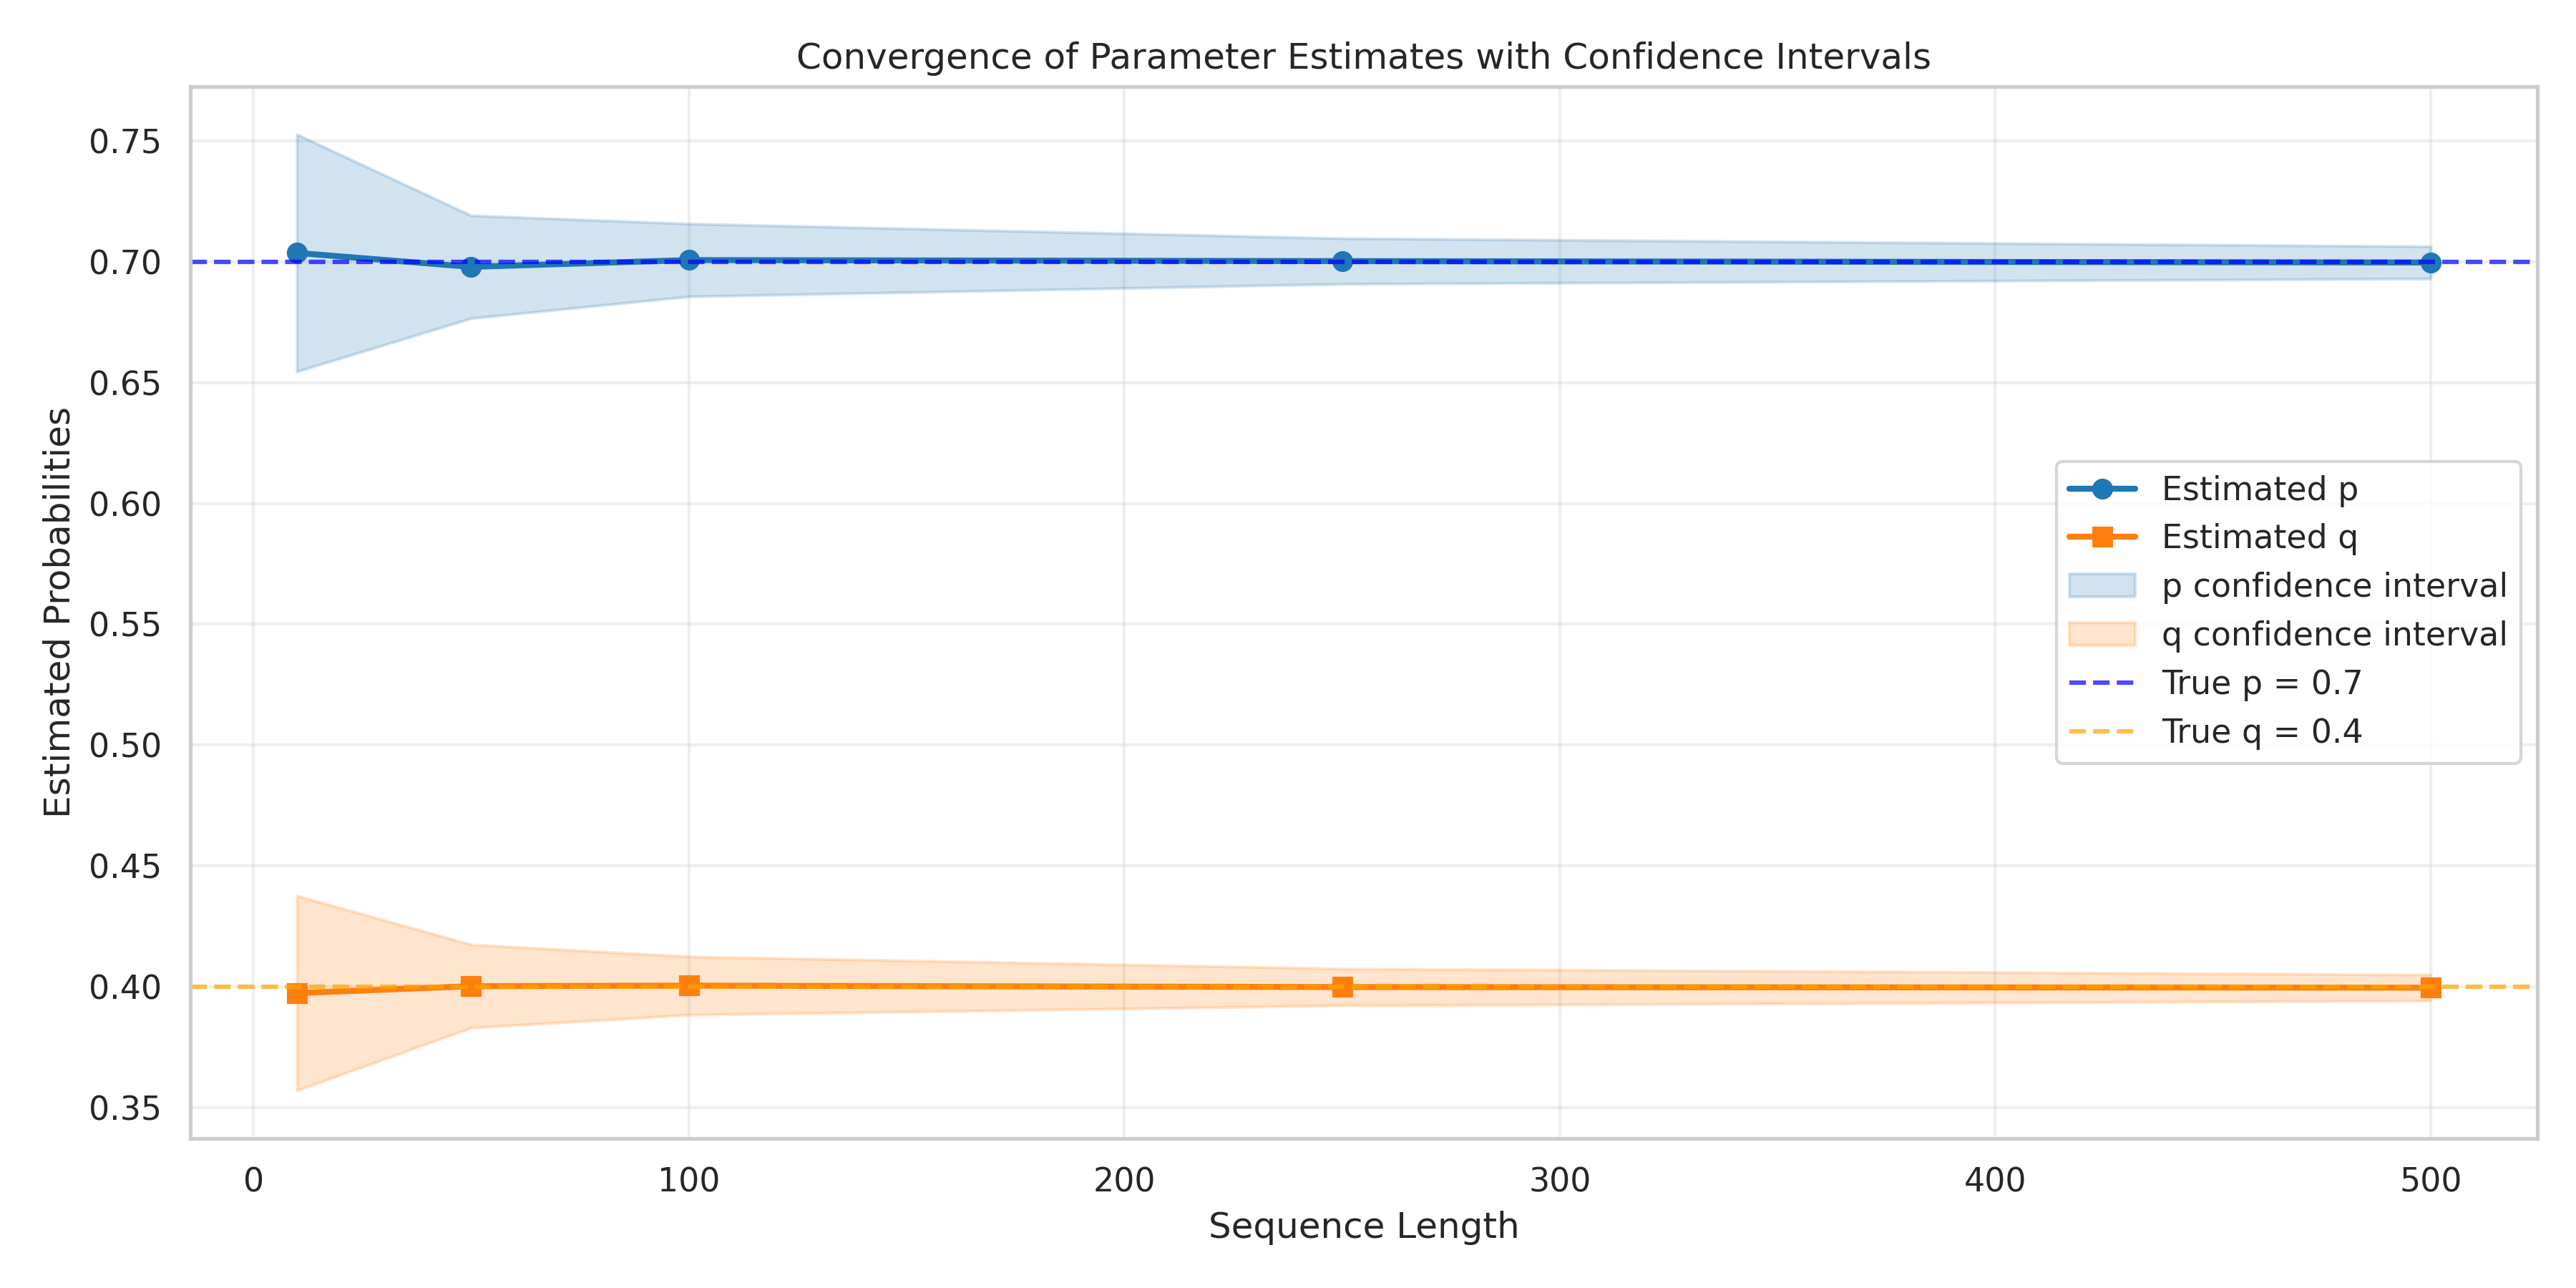
\includegraphics[width=\linewidth]{../DTMC/plots/convergence_plot_MLE_sequences.png}
  \caption{\footnotesize{Convergence of the MLE estimates for $p$ and $q$ with increasing size of traces (number of traces fixed to 100)}}
  \label{fig:convergence_plot_MLE_sequences}
\end{minipage}
\hfill
\begin{minipage}[b]{0.48\columnwidth}
  \centering
  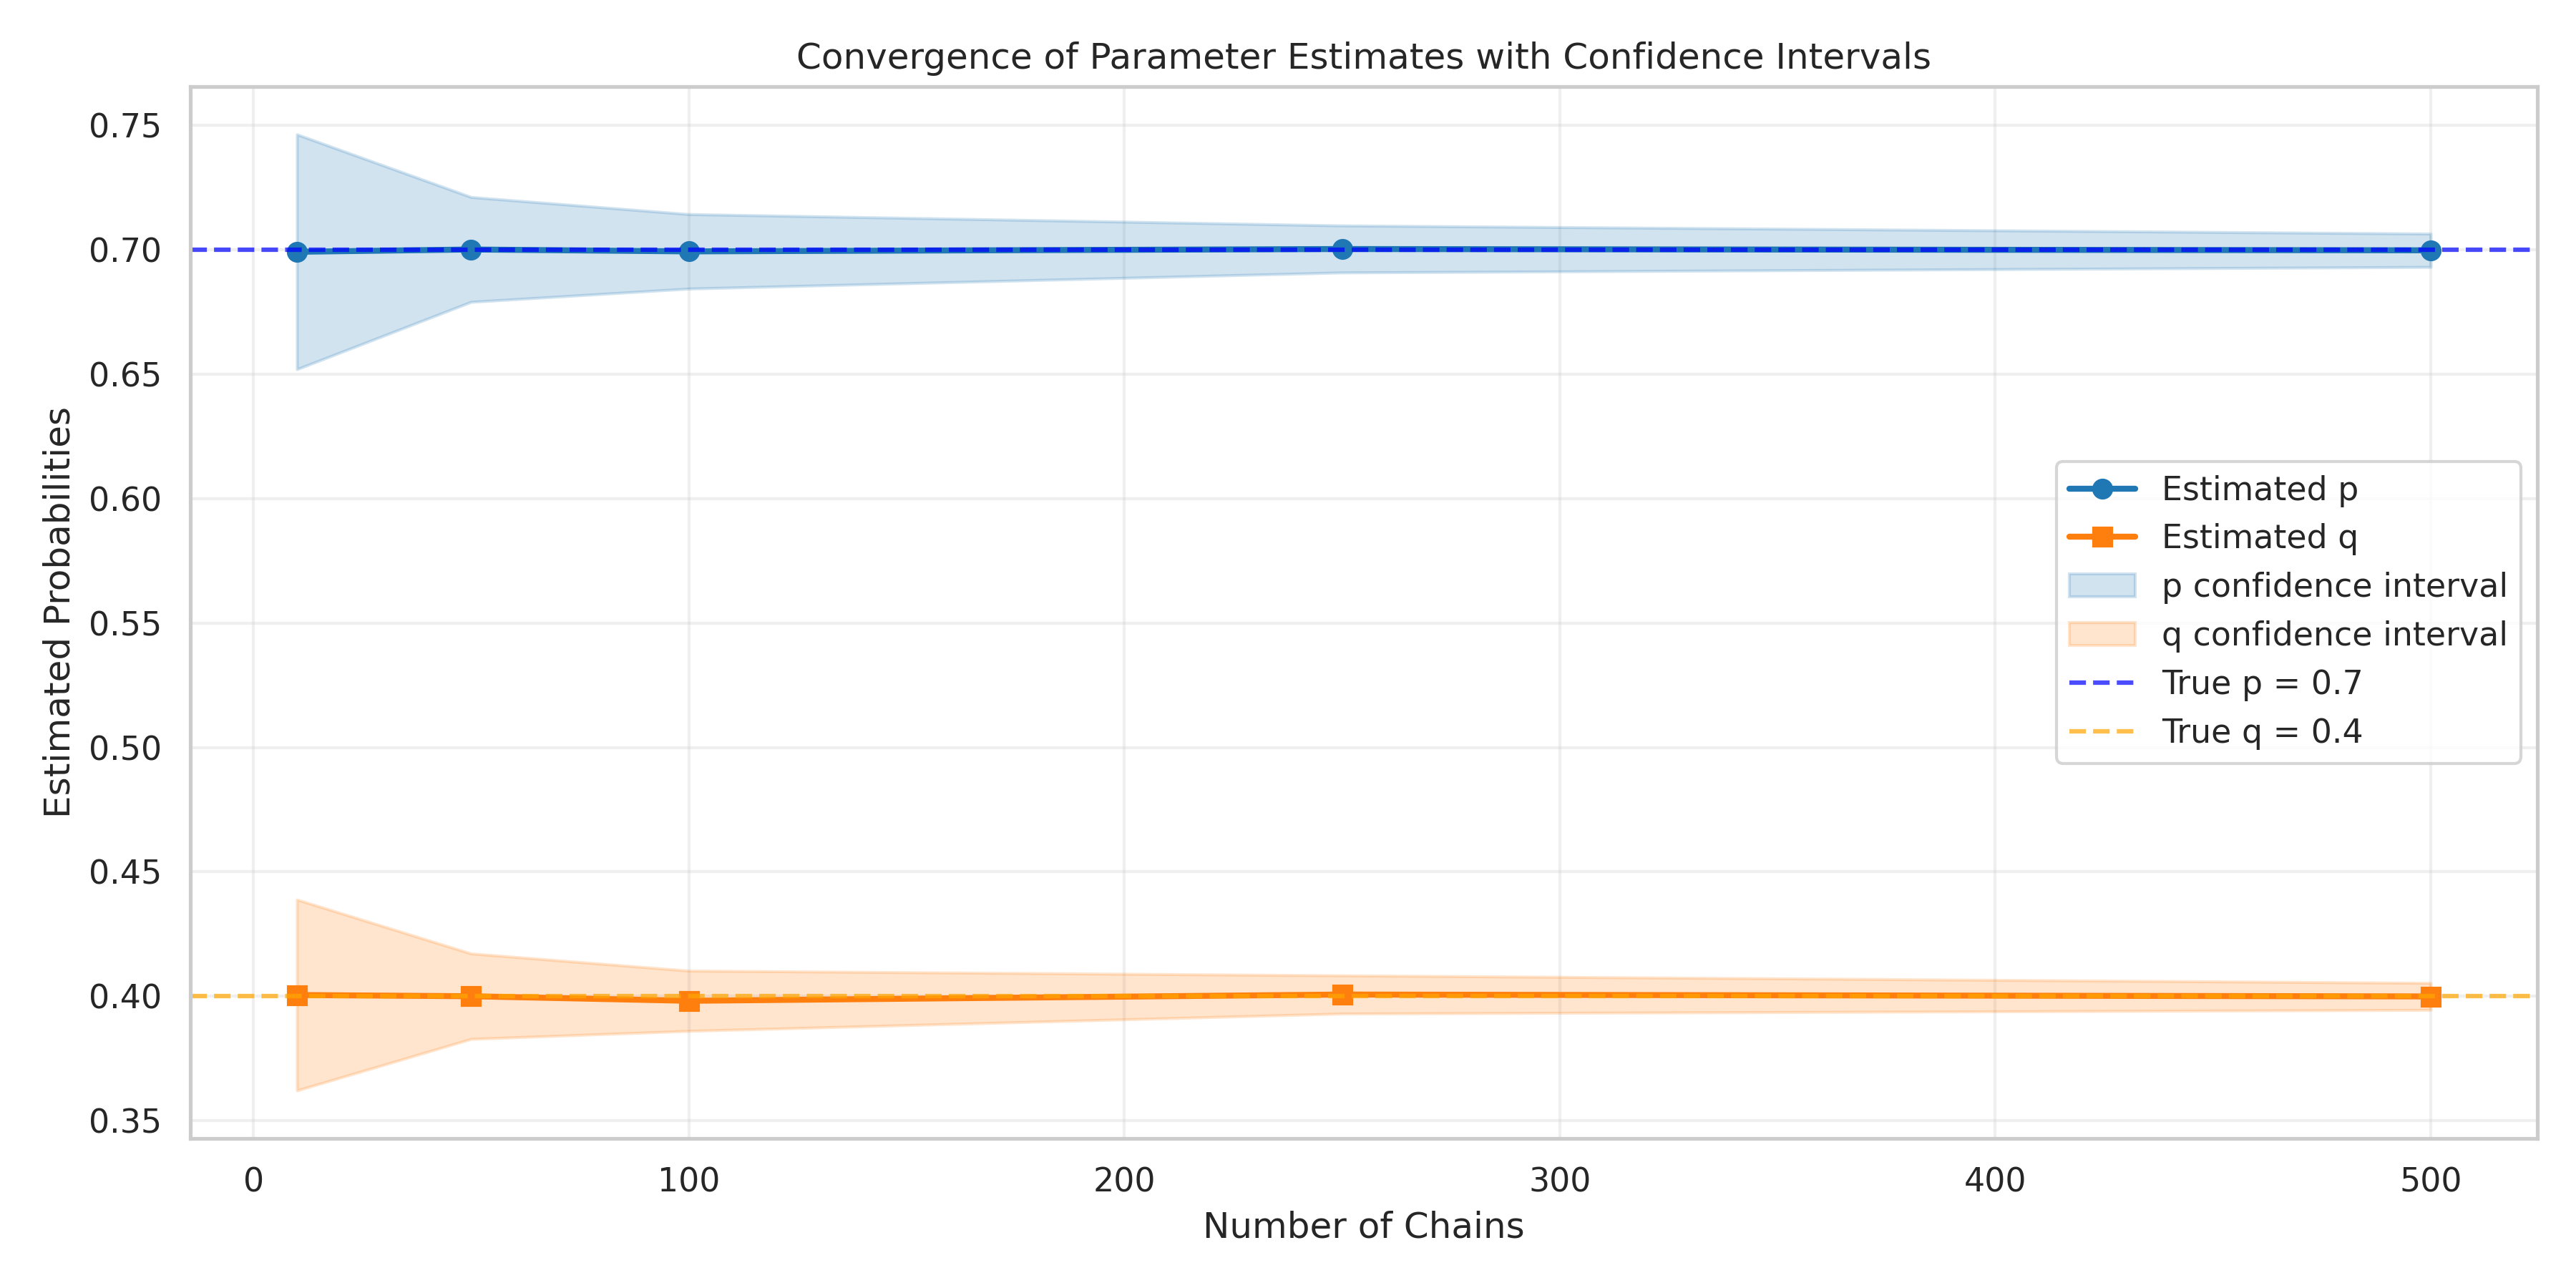
\includegraphics[width=\linewidth]{../DTMC/plots/convergence_plot_MLE_chains.png}
  \caption{\footnotesize{Convergence of the MLE estimates for $p$ and $q$ with increasing number of traces (length of traces fixed to 100)}}
  \label{fig:convergence_plot_MLE_chains}
\end{minipage}
\end{figure}

\begin{figure}[h]
\centering
  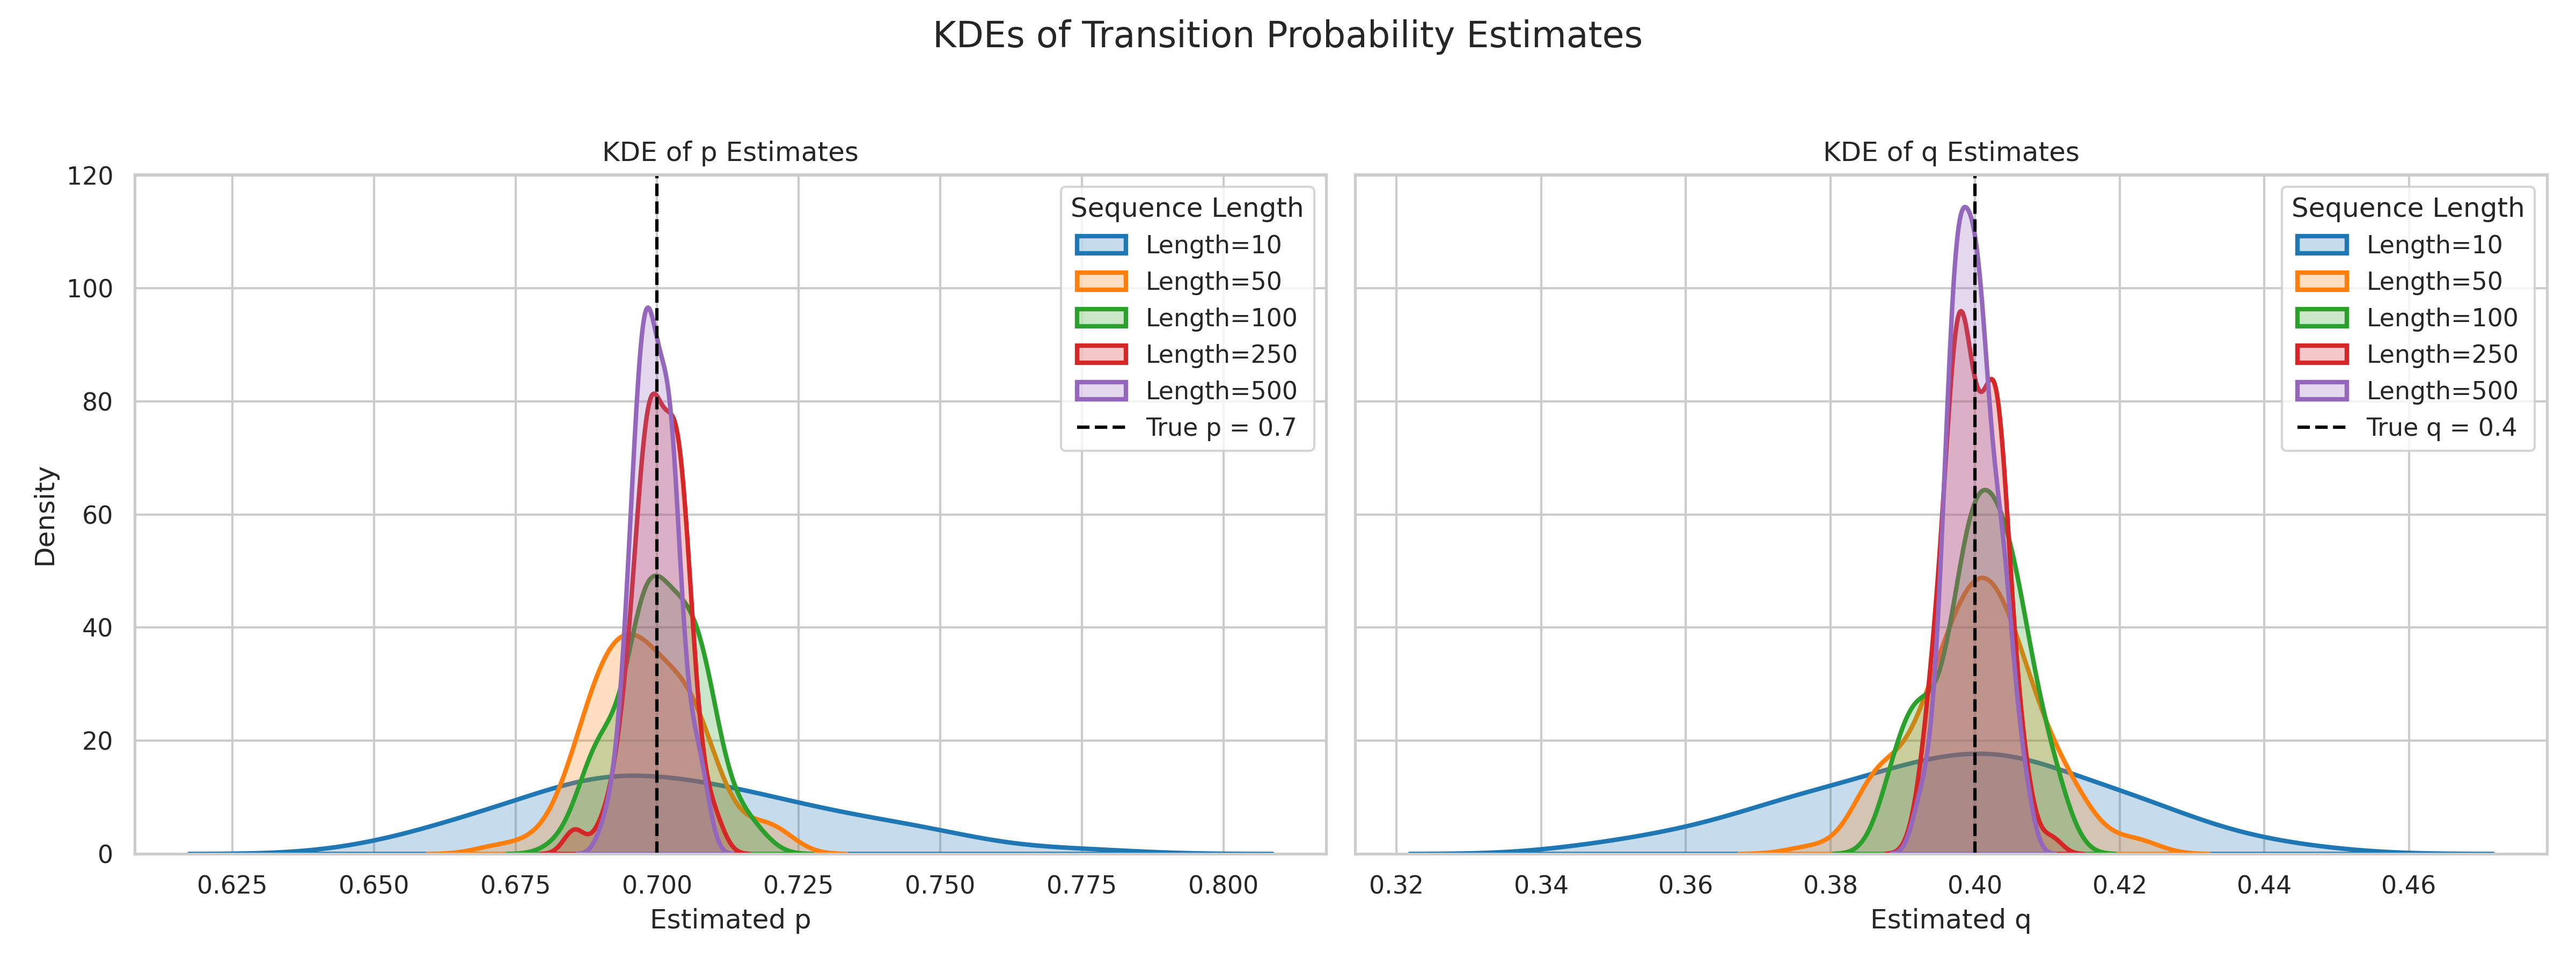
\includegraphics[width=\linewidth]{../DTMC/plots/kde_distributions_MLE_sequences.png}
  \caption{\footnotesize{Distribution of the MLE estimates for $p$ and $q$ with increasing size of traces (length of traces fixed to 100)}}
  \label{fig:distribution_plot_MLE_sequences}
\end{figure}

%questo secondo me è di troppo, perché il comportamento analogo lo abbiamo sulla convergenza
% \begin{figure}[h]
% \centering
%   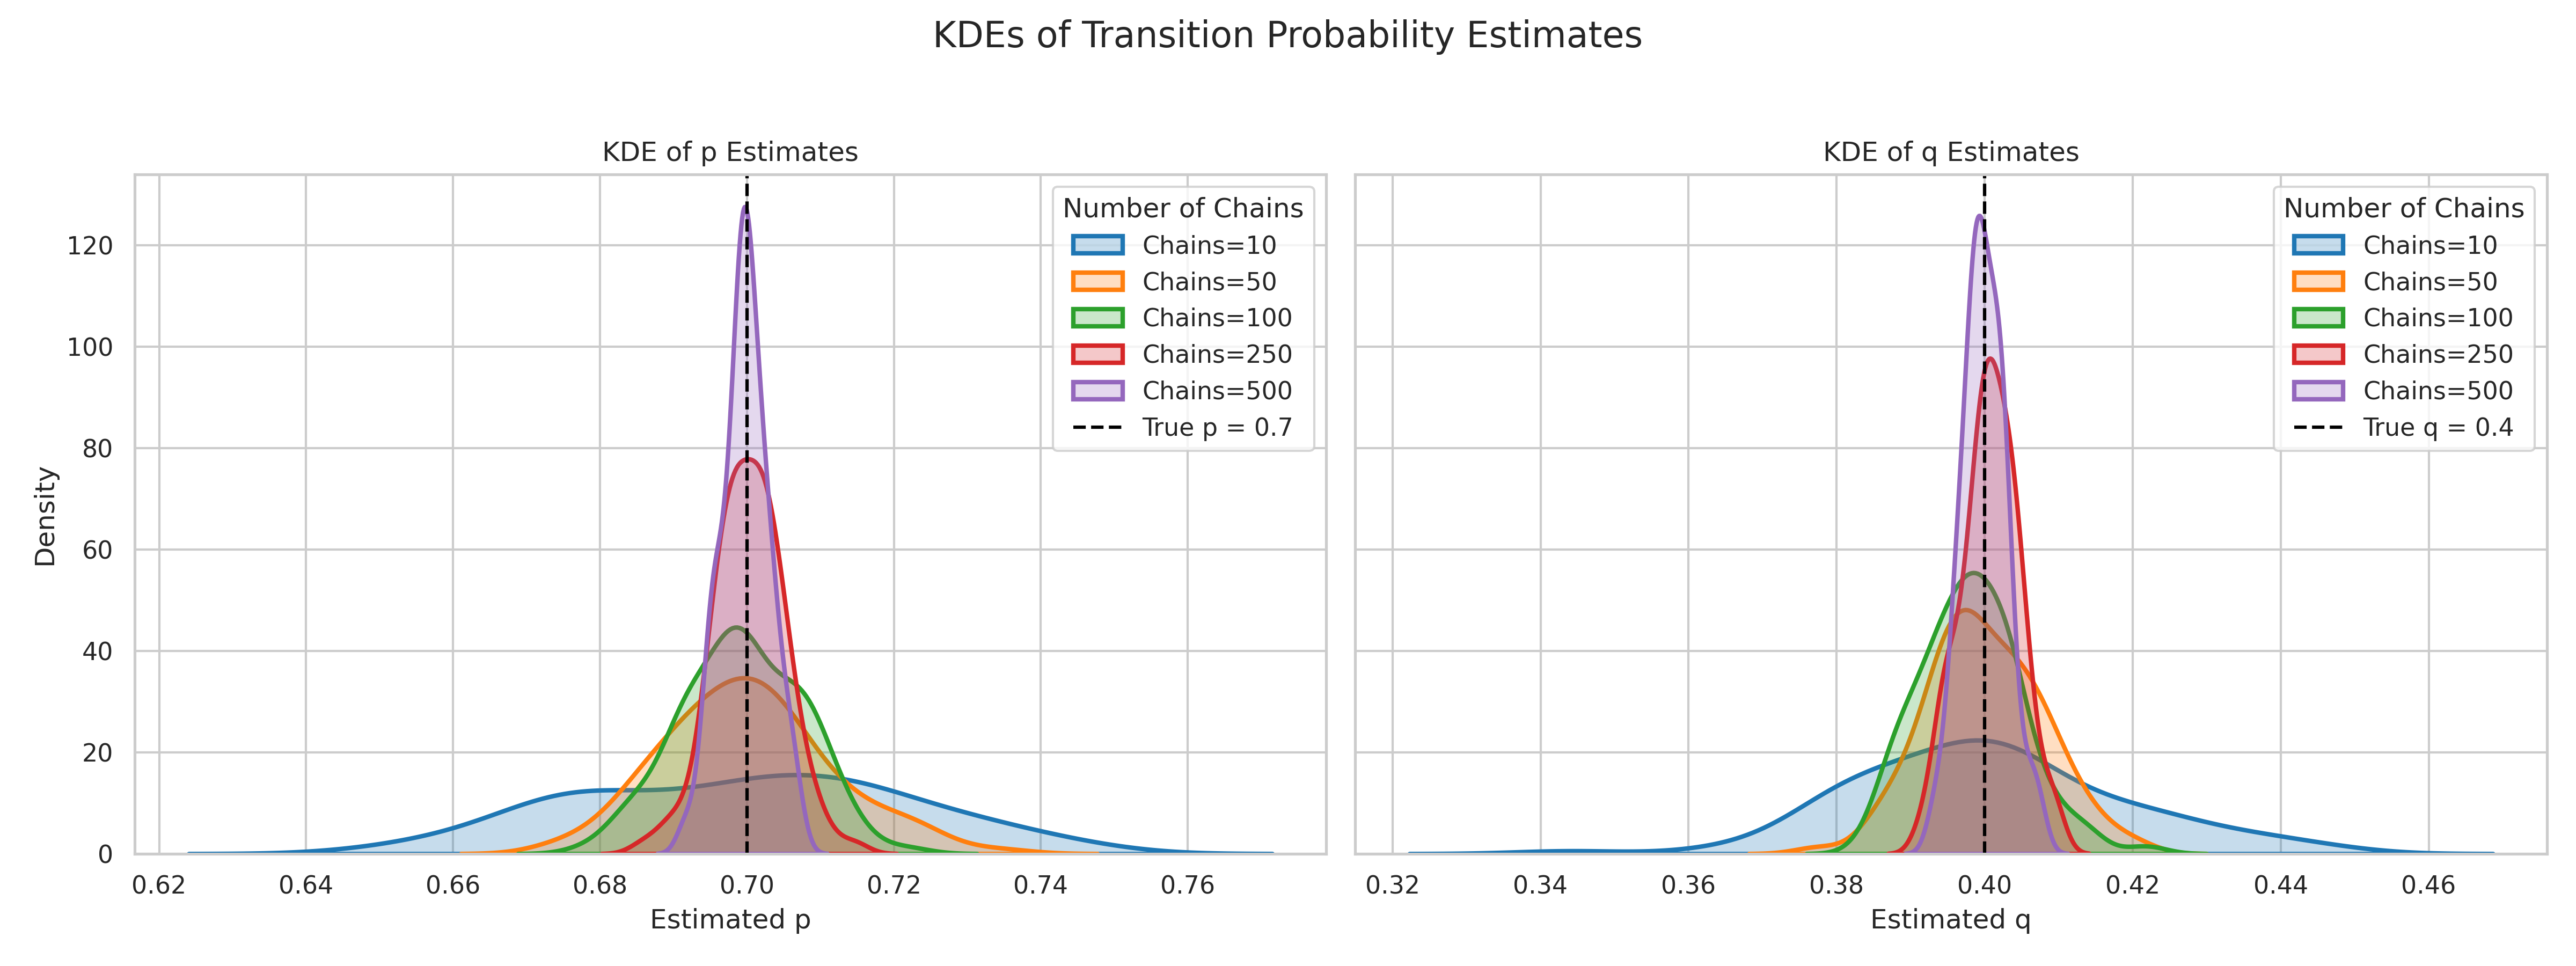
\includegraphics[width=\linewidth]{../DTMC/plots/kde_plot_MLE_chains.png}
%   \caption{\footnotesize{Distribution of the MLE estimates for $p$ and $q$ with increasing number of traces}}
%   \label{fig:distribution_plot_MLE_chains}
% \end{figure}

\begin{figure}[ht]
\centering
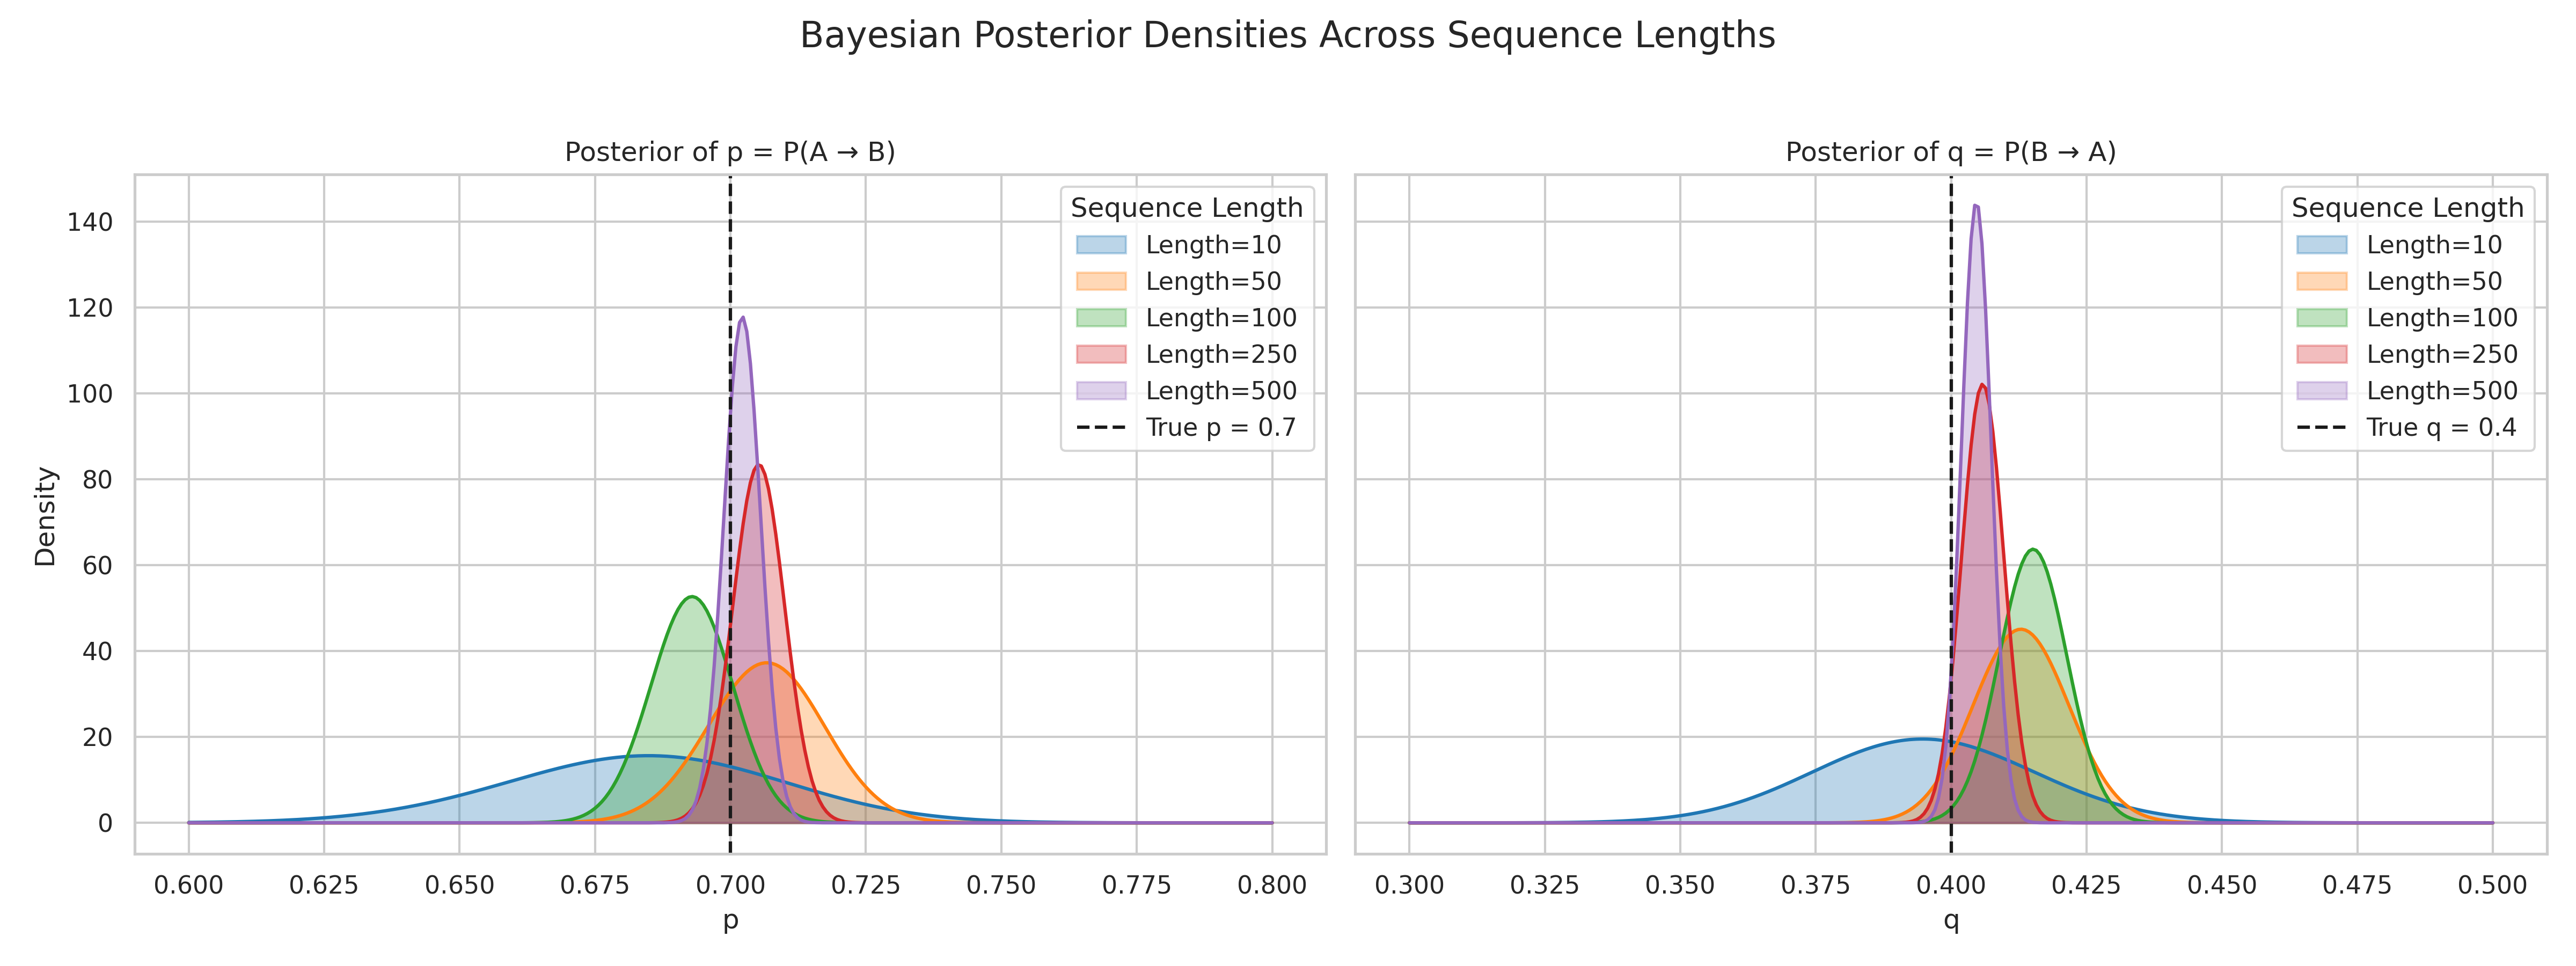
\includegraphics[width=\linewidth]{../DTMC/plots/posterior_distribution_sequences.png}
\caption{\footnotesize{Distribution of the Bayesian estimates for $p$ and $q$ with increasing size of traces (length of traces fixed to 100)}}
\label{fig:distribution_plot_Bayesian_sequences}
\end{figure}

% Anche questo per lo stesso motivo di prima, non lo metterei
% \begin{figure}[ht]
% \centering
% 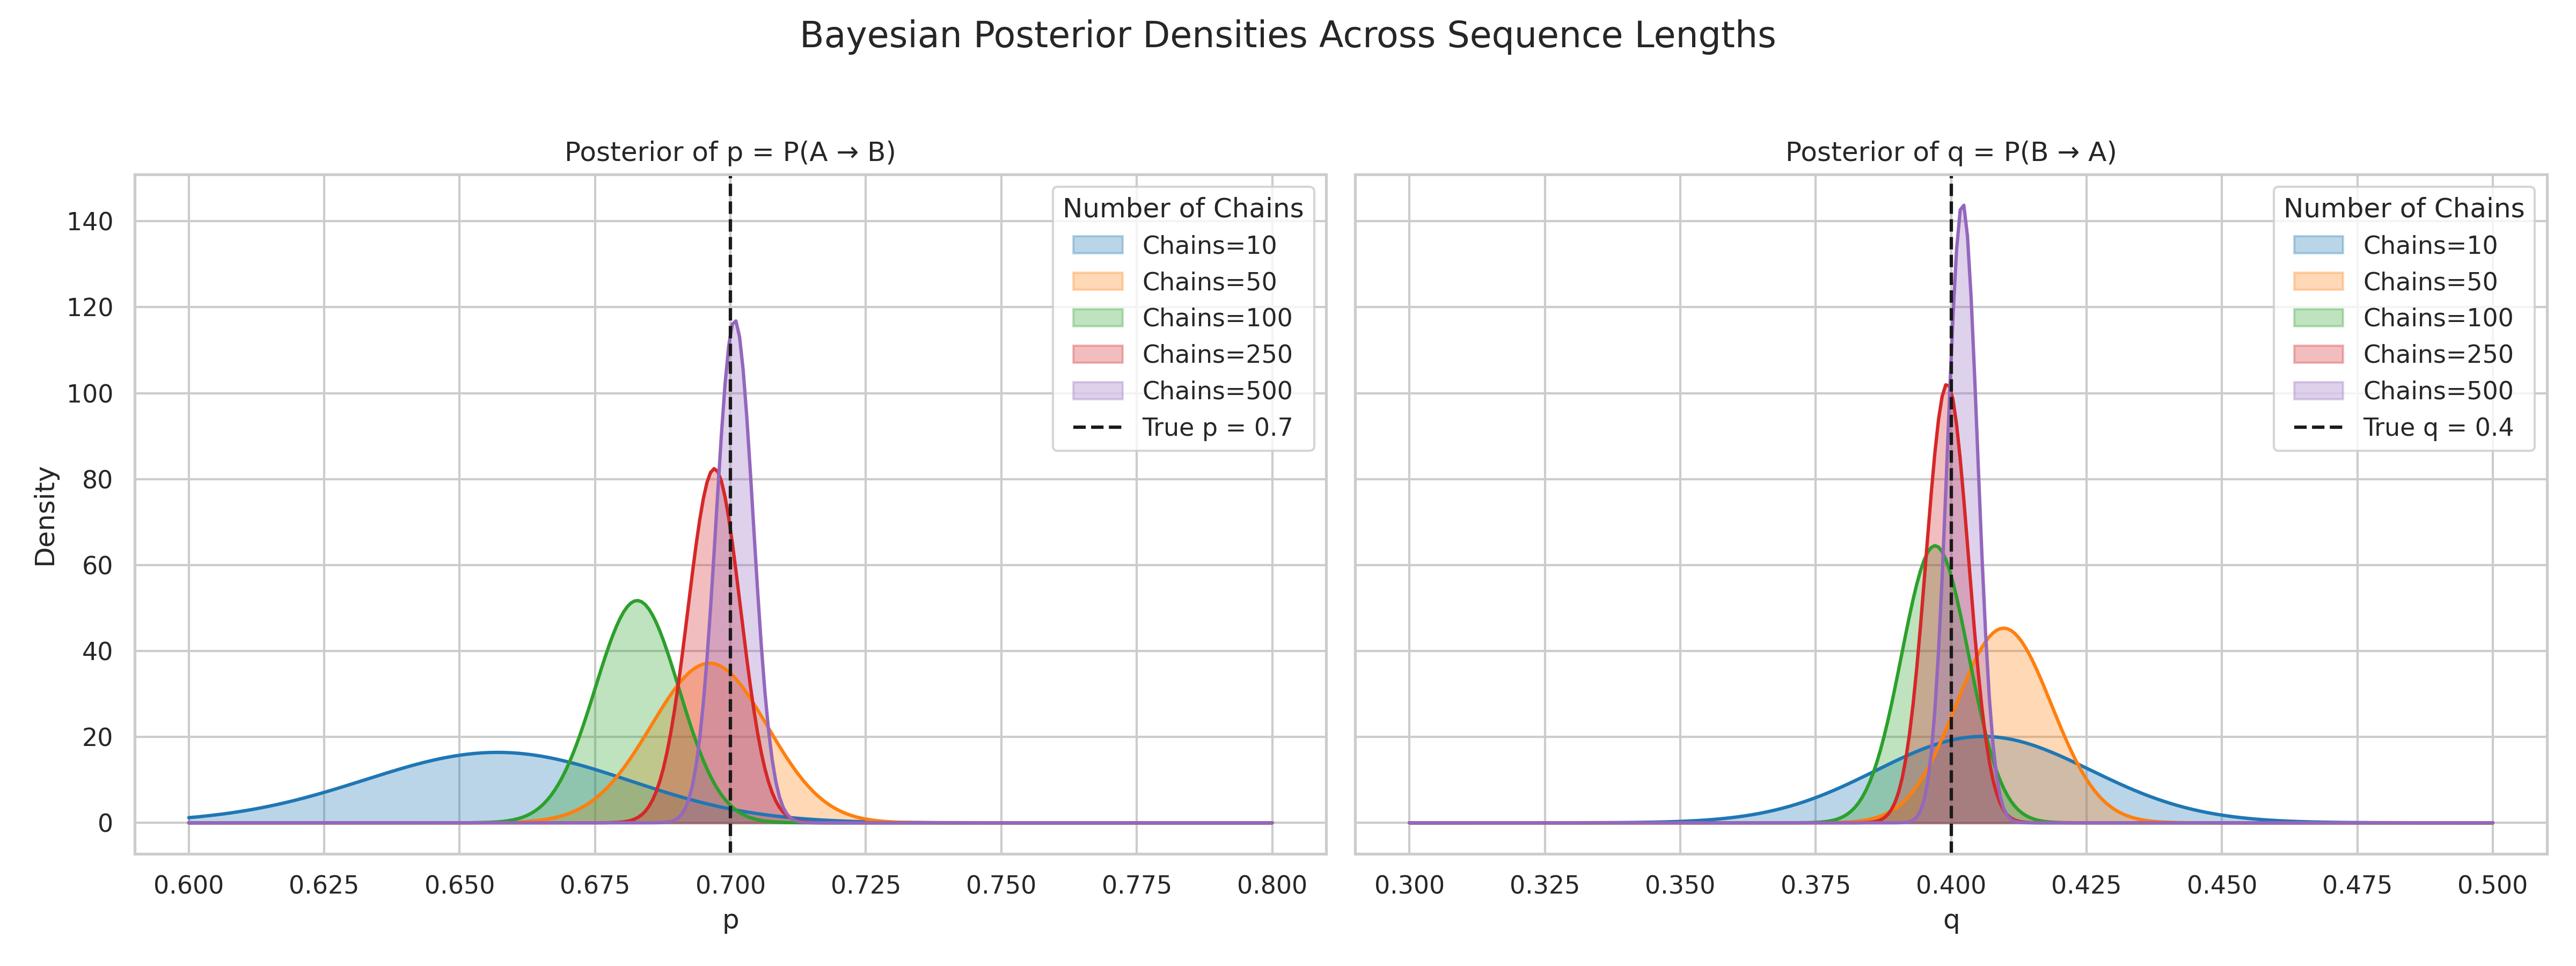
\includegraphics[width=\linewidth]{../DTMC/plots/posterior_distribution_chains.png}
% \caption{\footnotesize{Distribution of the Bayesian estimates for $p$ and $q$ with increasing number of traces}}
% \label{fig:distribution_plot_Bayesian_chains}
% \end{figure}
The number of observations highly impacts the quality of the results, both in terms of point estimates and confidence of the estimates.
Bayesian estimates are more stable and less affected by the number of observations, as they are able to adapt to the observed data and provide a more robust estimate of the parameters.

\subsection{Conclusions and considerations}
From our simulations, we conclude that ML estimation is very efficient, as the solution can be found analytically, but suffers
in terms of precision when the number of samples is low ($\leq 10000$ samples).
A Bayesian approach using conjugate priors may be more appropriate, as it allows the estimates to adapt dynamically to new observations (online learning framework).
This method becomes particularly effective when prior knowledge about the process parameters is available, guiding the inference towards faster convergence.\\[0.2cm]

In a more general framework of a DTMC with $|S|$ states, ML estimates are given by:
\begin{align*}
    \hat p_{ij} &= \frac{N_{ij}}{N_i} \;\;\forall i,j = 1, \dots, |S|
\end{align*}
where $N_{ij}$ is the number of transitions from state $s_i$ to state $s_j$, and $N_i = \sum_j N_{ij}$ is the total number of transitions from state $s_i$.
This simple generalization makes this approach very efficient, as the ML estimates can be computed in linear time with respect to the number of states and transitions.

Concerning confidence intervals, however, the approach is not that straight-forward. Goodman et al \cite{goodman1965paper}
showed that a general form of the ML confidence interval can be obtained when describing the DTMC changes of state with a Multinomial distribution.
The following expression holds $ \forall \; i,j=1, \dots, |S|$:
\begin{align*}
    \left[\frac{\chi^2_{\frac{1-\gamma}{|S|}, |S|-1} + 2N_{ij} -c}{2(N_i + \chi^2_{\frac{1-\gamma}{|S|}, |S|-1})} \leq \hat p_{ij} \leq \frac{\chi^2_{\frac{1-\gamma}{|S|}, |S|-1} + 2N_{ij} + c}{2(N_i + \chi^2_{\frac{1-\gamma}{|S|}, |S|-1})}\right]
\end{align*}
with $c = \sqrt{\chi^2_{\frac{1-\gamma}{|S|}, |S|-1} \left(\chi^2_{\frac{1-\gamma}{|S|}, |S|-1} + 4 N_{ij}\frac{(N_i - N_{ij})}{N_i}\right)}$, and 
$\chi^2_{\frac{1-\gamma}{|S|}, |S|-1}$ being the Chi-Squared quantile with $|S| - 1$ degrees of freedom and confidence level $\frac{1 - \gamma}{|S|}$.\\[0.1cm]

From a Bayesian perspective, conjugate prior families can still be leveraged when analytical tractability is desired. Modeling state 
transitions with a Categorical distribution pairs naturally with the Dirichlet distribution as a conjugate prior, 
allowing for closed-form posterior updates. However, alternative modeling strategies that do not rely on conjugate relationships (such as more 
flexible prior specifications or more complex hierarchical structures) may necessitate approximate inference methods such as Markov Chain Monte 
Carlo (MCMC) or Variational Inference.

\newpage

\section{Multi-Agent Reinforcement Learning on Stochastic Game}
In this section, we present the design and implementation of a multi-agent reinforcement learning (MARL) algorithm in a two-player zero-sum stochastic game setting. 
The environment is based on the simplified soccer game, originally proposed by Littman in \cite{littman1994markov}.
\subsection{Environment}
The environment consists of a 4×5 grid populated by two players, each of whom can choose to move up, down, left, right, or remain stationary at each step. Ball possession is initially assigned at random. Both players 
select their actions simultaneously, which are then executed in a randomly determined order. Ball possession plays a central role in the game 
dynamics: when a player attempts to move into the square currently occupied by the opponent, possession is transferred to 
the invaded player, while the invading player's move is canceled. A player scores by reaching the opponent's goal area 
when in possession of the ball, receiving a reward of +1 (the opponent incurs a penalty of -1 instead). At the beginning of each match, 
the players are positioned as shown in Figure~\ref{fig:game_scheme}, with ball possession assigned randomly.
\begin{figure}[h]
    \caption{\footnotesize{Game scheme}}
    \centering
    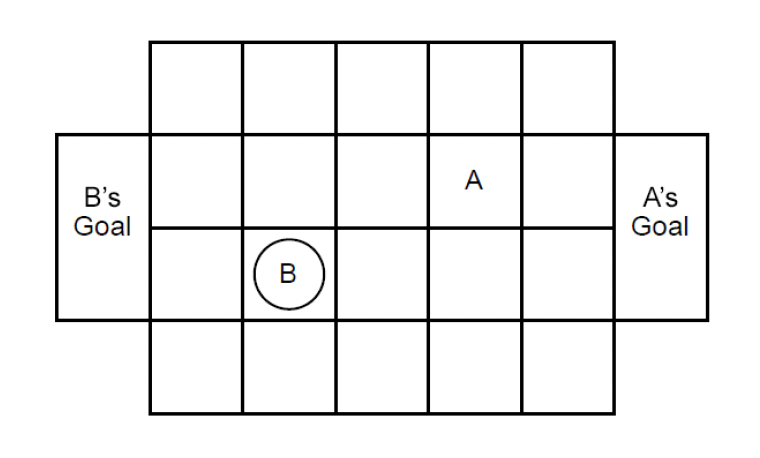
\includegraphics[width=0.28\textwidth]{../assets/game_scheme.png}
    \label{fig:game_scheme}
\end{figure}

\subsection{Learning algorithm}
The implemented approach is a belief-based joint action learning algorithm that employs behavioral strategies. \emph{Behavioral} refers to the fact that 
actions are sampled from a probability distribution, rather than being selected via a deterministic policy. The \emph{belief} component indicates that, over the 
course of the game, each player continuously updates an estimate of the opponent’s action distribution. The learning process extends the standard version of Q-learning with the 
following update steps (w.r.t one of the two agents):

\textbf{Q-value update}
    \begin{flalign*}
        Q_{t+1}(s_t, a_t, o_t) &= (1-\alpha_t) Q_t(s_t, a_t,o_t) + \alpha_t \left( r_t + \gamma V_t(s_{t+1}) \right)
    \end{flalign*}

\textbf{Policy update} (using linear programming)
    \begin{flalign*}
        \pi_{t+1}(s_t) &= \arg\max_{\pi_t(s_t)} \sum_{a_t,o_t} \pi_t(s_t)[a_t] B_{t+1}(s_t,o_t)Q_{t+1}(s_t, a_t,o_t)
    \end{flalign*}

\textbf{Utility update}
    \begin{flalign*}
        V_{t+1}(s_t) &= \max_{a_t} \sum_{a_t,o_t} \pi_{t+1}(s_t)[a_t] B_{t+1}(s_t,o_t) Q_{t+1}(s_t, a_t,o_t)
    \end{flalign*}

where $s_t$ is the joint current state of the game, $a_t$ is the action taken by the agent, $o_t$ is the opponent's action.

As a belief function, we use a probability distribution over the opponent’s actions conditioned on the current state. This distribution is updated in an online fashion throughout the game, 
incorporating the opponent’s observed actions to refine the estimate over time.

\subsection{Experiments \& Results}
% The algorithm was learned in $10^6$ moves, with the following parameters:
% \begin{itemize}
%     \item $\alpha_0 = 1$
%     \item $\alpha_{t+1} = \alpha_t *10^{\log_{10} \frac{0.01}{10^6}}$
%     \item $\gamma = 0.9$
%     \item $\epsilon = 0.2$
% \end{itemize}

% Training was conducted using two approaches: against a random opponent and in a self-play setup with simultaneous learning. Performance was evaluated over $10^5$
% test moves against both types of opponents, with each test repeated 10 times and average results recorded. In tests with draw conditions enabled, games ended in a draw with a 0.1 probability. 
% Results are summarized in Table \ref{tab:results}.
The learning task was carried out under two settings: (i) against a random opponent, and (ii) in self-play against another learner of identical design. In both cases, training lasted for $10^6$ steps using the following parameters:
\begin{align*}
    \alpha_0 &= 1 \\
    \alpha_{t+1} &= \alpha_t \cdot 10^{\log_{10} \left( \frac{0.01}{10^6} \right)} \\
    \gamma &= 0.9 \\
    \epsilon &= 0.2
\end{align*}

After training, the learned strategies were evaluated over $10^5$ test steps. Besides standard testing, an additional setting was considered in which the game could terminate early 
at each step with probability $1 - \gamma = 0.1$, resulting in a draw (zero reward to both players) and immediate reset of
 the environment. This mechanism emulates the effect of the discount factor $\gamma$ during evaluation. Due to the 
 stochastic nature of the process, the entire training and testing routine was repeated 10 times for robustness.
 Performance metrics are reported as 95\% confidence intervals. Results are summarized in Tables \ref{tab:result1} and \ref{tab:result2}, with the following legend on the settings:
 ``random" and ``belief" refer to the opponent's strategy while training, while ``dummy" refers to a fixed strategy that always perform a random action.
%  \begin{table}[h]
% \centering
% \caption{Results of the test}
% \label{tab:results}
% \begin{tabular}{|c|c|c|}
%     ...
% \end{tabular}
% \end{table}
\begin{table}[h!]
    \centering
    \scalebox{0.85}{
        \begin{tabular}{lccc}
            Setting & Home Win \%  & Matches & Avg. Len. \\
            \hline 
            random-dummy &  $94.51 \pm 0.67 \%$  & $8351.40 \pm 432.02$ & $12.03 \pm 0.65$ \\
            belief$_A$-belief$_B$ & $53.51 \pm 4.08 \%$  & $8454.60 \pm 1071.30$ & $12.20 \pm 1.69$ \\
            belief$_A$-dummy & $89.42 \pm 1.33 \%$  & $4422.20 \pm 472.39$ & $23.03 \pm 2.28$ \\
            dummy-belief$_B$ & $12.12 \pm 1.08 \%$ & $3824.30 \pm 390.25$ & $26.57 \pm 2.40$ \\
            \hline 
        \end{tabular}
        }
        \caption{Results without early termination}
        \label{tab:result1}
\end{table}

\begin{table}[h!]
    \centering
    \scalebox{0.85}{
        \begin{tabular}{lccc}
            Setting & Home Win \% &  Matches & Avg. Len. \\
            \hline 
            random-dummy &  $97.74 \pm 0.36 \%$  & $6343.10 \pm 542.92$ & $7.44 \pm 0.45$ \\
            belief$_A$-belief$_B$ & $56.87  \pm 7.67 \%$ & $5886.50 \pm 1276.90$ & $8.42 \pm 1.17$ \\
            belief$_A$-dummy & $95.21 \pm 1.02 \%$  & $3304.30 \pm 720.17$ & $9.72 \pm 1.31$ \\
            dummy-belief$_B$ & $6.61 \pm 1.18 \%$  & $2581.90 \pm 513.34$ & $10.79 \pm 1.03$ \\
            \hline 
        \end{tabular}
        }
        \caption{Results with early termination}
        \label{tab:result2}
\end{table}

\subsection{Conclusion}
The belief-based joint action learning algorithm exhibits strong adaptive capabilities across diverse opponent strategies in the stochastic soccer domain. 
The algorithm is able to learn a good strategy against a random opponent, achieving an expected win rate percentage of $94.51 \pm 0.67$ and an expected average match length of $12.03 \pm 0.65$ steps.
When training is performed via self-play, the win rate against a random opponent slightly decreases ($89.42 \pm 1.33$), while the 
average match length increases ($23.03 \pm 2.28$). This phenomenon might be likely due to the lack of strategy in the random opponent, which can lead to atypical scenarios 
that were underrepresented during learning, challenging the trained agent. Moreover, the near perfect equilibrium achieved in self-play, with a win rate of $53.51 \pm 4.08$, provides strong empirical evidence of convergence to an optimal strategy for both the agents.

Lastly, the sensitivity of estimates to early termination reveals important considerations about the role of temporal horizons. The marked improvement in performance 
against a random opponent, coupled with the stable results against a belief-based opponent, suggests that the effective discount factor plays 
a crucial role in shaping the learning dynamics by enhancing the agent's preference for shorter and more decisive actions.
\onecolumn
\newpage
\nocite{*}
\bibliographystyle{plain}
\bibliography{mas_report}

\end{document}